\clearpage
\section{Motorcontroller}

The chassis used for the rover has 4 pre-installed DC motors, which are used for movement. To control the direction of the rover a Sabertooth 2x5 motor controller has been connected to the motors. The motor controller is used to operate the steering, forward and reversing actions of the rover.

\begin{figure}[H]
	\centering
	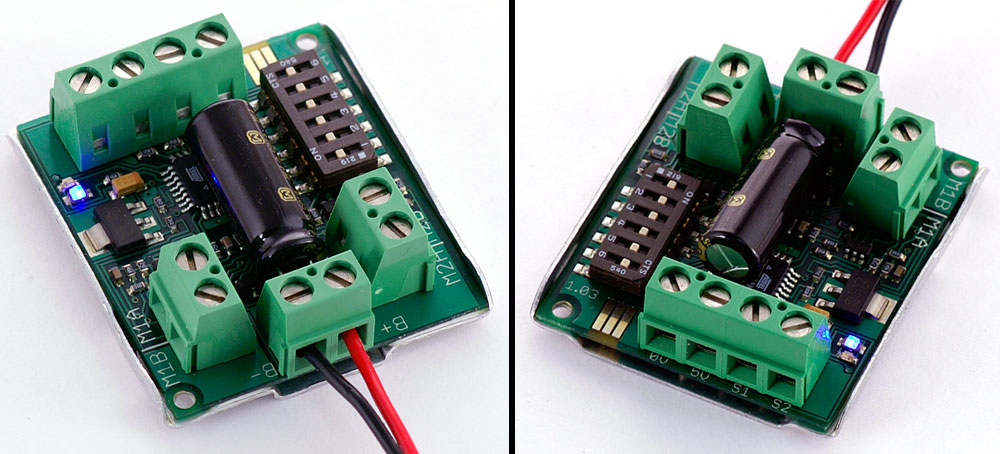
\includegraphics[width=.8\linewidth]{images/Sabertooth2X5big.jpg}
	\caption{Sabertooth 2x5\cite{sabertoothpic}}
\end{figure}

The driver uses a 5V supply to operate, which is easily supplied by the Raspberry Pi that is used to control the entire rover. The board supports two separate DC motor outputs that can independently controlled, in this case two motors will be connected to either side.

%Talk about how the signalling works
%Possibly add a diagram

%http://www.dimensionengineering.com/datasheets/Sabertooth2X5QuickStart.pdf
%http://www.dimensionengineering.com/datasheets/Sabertooth2x5.pdf
%http://www.dimensionengineering.com/products/sabertooth2x5